\documentclass[a4paper,12pt]{article}

\usepackage[english]{babel}
\usepackage[T1]{fontenc}
%\usepackage[utf8]{inputenc}

\usepackage[
  left=20mm,
  right=20mm,
  top=22mm,
  bottom=22mm,
  headheight=16pt,
  headsep=10mm
]{geometry}

\usepackage{graphicx}
\usepackage{float}
\usepackage{booktabs}
\usepackage{tabularx}
\usepackage{array}
\usepackage{multirow}
\usepackage{fancyhdr}
\usepackage{mwe}

\usepackage{booktabs}
\usepackage{array}

\pagestyle{fancy}
\fancyhf{}
\renewcommand{\headrulewidth}{0.4pt}
\renewcommand{\footrulewidth}{0pt}
\fancyfoot[C]{\thepage}

\newenvironment{fullwidth}{\begin{minipage}{\textwidth}}{\end{minipage}}

\newcommand{\reporttitle}{CAELI: Climate-smArt dEcision for a rEsiLient avIation}
\newcommand{\reportsubtitle}{Bollettino mensile di previsione stagionale per il supporto alle operazioni con droni}
\newcommand{\reportauthors}{Amigo srl}
\newcommand{\reportdate}{\today}

\fancyhead[R]{}
\fancyhead[L]{}

%----------------------------------------------------------------------------------------

\begin{document}

\newcommand{\MONTHone}{March 2026}
\newcommand{\MONTHtwo}{May 2026}

\newcommand{\AMIGO}{logo.png}
\newcommand{\FIGCALENDAR}{fig_calendar.png}
\newcommand{\FIGAREAONE}{fig_area1.png}
\newcommand{\FIGAREATWO}{fig_area2.png}
\newcommand{\FIGAREATHREE}{fig_area3.png}
\newcommand{\FIGRISKS}{fig_risks.png}

\IfFileExists{logo.png}{}{\renewcommand{\AMIGO}{example-image}}
\IfFileExists{fig_calendar.png}{}{\renewcommand{\FIGCALENDAR}{example-image}}
\IfFileExists{fig_area1.png}{}{\renewcommand{\FIGAREAONE}{example-image}}
\IfFileExists{fig_area2.png}{}{\renewcommand{\FIGAREATWO}{example-image}}
\IfFileExists{fig_area3.png}{}{\renewcommand{\FIGAREATHREE}{example-image}}
\IfFileExists{fig_risks.png}{}{\renewcommand{\FIGRISKS}{example-image}}

%----------------------------------------------------------------------------------------
% TITLE PAGE
%----------------------------------------------------------------------------------------

\thispagestyle{empty}

\begin{fullwidth}
\vspace*{-0.075\textheight}

\noindent\includegraphics[width=0.35\textwidth]{\AMIGO}

\vspace{0.15\textheight}

{\raggedright\fontsize{50pt}{52pt}\selectfont\textbf{\reporttitle}\par}

\vspace{0.03\textheight}

{\LARGE\textit{\textbf{\reportsubtitle}}\par}

\vfill

{\Large\reportauthors\par}

\vfill\vfill\vfill

{\large\reportdate\par}
\end{fullwidth}

\newpage

%----------------------------------------------------------------------------------------
% DISCLAIMER PAGE
%----------------------------------------------------------------------------------------

\thispagestyle{empty}
\footnotesize

\subsection*{Disclaimer}
Bla bla bla

\subsection*{Copyright}
\textcopyright\ [2026] [Amigo srl]

\subsection*{Contact}
Via Flaminia, 48, 00196 Rome, Italy

sara.dalgesso@amigoclimate.com

\vfill

\subsubsection*{Changelog}
\scriptsize

\begin{tabular}{@{} p{0.08\linewidth} p{0.18\linewidth} p{0.70\linewidth} @{}}
\toprule
v1.0 & 2026-03-13 & First version, agreed in a preliminary discussion with the client \\
\bottomrule
\end{tabular}

\newpage

%----------------------------------------------------------------------------------------
% BULLETIN
%----------------------------------------------------------------------------------------

\normalsize

\section{Sintesi}
Le previsioni stagionali relative al periodo marzo 2026 -- maggio 2026 indicano che:
\begin{itemize}
  \item bla bla
  \item bla bla
\end{itemize}

\section{Dati e metodologia}
Il servizio CAELI fornisce bollettini mensili basati sulle previsioni stagionali del sistema Seasonal Forecast System version 5 (SEAS5) del Centro Europeo per le Previsioni Meteorologiche a Medio Termine (ECMWF). Le analisi sono prodotte per sette aree corrispondenti ad altrettante regioni italiane, riportate nella Tabella~\ref{tab:regioni_aree}. 

I dataset utilizzati sono stati elaborati mediante le metodologie proprietarie di downscaling statistico e bias correction sviluppate da Amigo, al fine di aumentare la risoluzione spaziale fino a $5.5\,\mathrm{km}$ e migliorare la rappresentatività delle condizioni meteorologiche a scala locale. Le specifiche relative alle variabili meteorologiche considerate, ai dataset di partenza e alle procedure di elaborazione applicate sono descritte nell’Allegato Tecnico del servizio, che fornisce ulteriori dettagli sul funzionamento dell’algoritmo di processamento dei dati.

A partire dalle variabili meteorologiche considerate sono stati definiti due indicatori operativi per valutare le condizioni meteorologiche favorevoli alle operazioni con droni. Il primo quantifica il numero di giorni con precipitazione giornaliera inferiore a $1\,\mathrm{mm}$, mentre il secondo indica il numero di giorni in cui la radiazione solare superficiale supera la soglia operativa di $600\,\mathrm{J\,m^{-2}}$. Gli indicatori esprimono quindi il numero di giorni, all’interno di ciascun mese, in cui le condizioni meteorologiche risultano compatibili con le operazioni di volo. 

I prodotti previsionali sono generati con una risoluzione spaziale finale di $5.5\,\mathrm{km}$ e sono forniti sia come valori aggregati mensili a scala regionale, ottenuti tramite media spaziale, sia come mappe regionali che descrivono la distribuzione spaziale degli indicatori operativi. Le mappe sono visualizzate su uno sfondo cartografico basato su OpenStreetMap (OSM), che consente di collocare i risultati nel relativo contesto geografico.

\begin{table}[H]
\centering
\begin{tabular}{ll}
\toprule
\textbf{Area} & \textbf{Regione} \\
\midrule
Area 1 & Abruzzo \\
Area 2 & Friuli Venezia Giulia \\
Area 3 & Lazio \\
Area 4 & Marche \\
Area 5 & Piemonte \\
Area 6 & Toscana \\
Area 7 & Umbria \\
\bottomrule
\end{tabular}
\caption{Corrispondenza tra le aree utilizzate nel bollettino e le regioni italiane considerate.}
\label{tab:regioni_aree}
\end{table}

%\section{Seasonal forecasts overview}
\section{Previsione aggregata}

La presente sezione riporta, per ciascuna delle sette regioni considerate, i valori aggregati degli indicatori operativi, espressi come calendario mensile.

\begin{figure}[H]
\centering
\includegraphics[width=0.95\textwidth]{figures/abruzzo_calendar.png}
\caption{Calendario del numero medio mensile di giorni adatti alle operazioni coi droni.}
\label{fig: calendar_abruzzo}
\end{figure}

\begin{figure}[H]
\centering
\includegraphics[width=0.95\textwidth]{figures/friuli_calendar.png}
\caption{Calendario del numero medio mensile di giorni adatti alle operazioni coi droni.}
\label{fig: calendar_friuli}
\end{figure}

\begin{figure}[H]
\centering
\includegraphics[width=0.95\textwidth]{figures/lazio_calendar.png}
\caption{Calendario del numero medio mensile di giorni adatti alle operazioni coi droni.}
\label{fig: calendar_lazio}
\end{figure}

\begin{figure}[H]
\centering
\includegraphics[width=0.95\textwidth]{figures/marche_calendar.png}
\caption{Calendario del numero medio mensile di giorni adatti alle operazioni coi droni.}
\label{fig: calendar_marche}
\end{figure}

\begin{figure}[H]
\centering
\includegraphics[width=0.95\textwidth]{figures/piemonte_calendar.png}
\caption{Calendario del numero medio mensile di giorni adatti alle operazioni coi droni.}
\label{fig: calendar_piemonte}
\end{figure}

\begin{figure}[H]
\centering
\includegraphics[width=0.95\textwidth]{figures/toscana_calendar.png}
\caption{Calendario del numero medio mensile di giorni adatti alle operazioni coi droni.}
\label{fig: calendar_toscana}
\end{figure}

\begin{figure}[H]
\centering
\includegraphics[width=0.95\textwidth]{figures/umbria_calendar.png}
\caption{Calendario del numero medio mensile di giorni adatti alle operazioni coi droni.}
\label{fig: calendar_umbria}
\end{figure}

%\section{Seasonal forecasts maps}
\section{Previsione regionale}
La presente sezione riporta le mappe degli indicatori operativi a $5.5\,\mathrm{km}$ per ciascuna delle sette regioni italiane considerate, per ogni mese di previsione.

\subsection{Abruzzo}
\begin{figure}[H]
\centering
\includegraphics[width=0.95\textwidth]{figures/rad/abruzzo_rad.png}
\caption{Mappa ad alta risoluzione ($5.5\,\mathrm{km}$) del numero medio di giorni con radiazione solare sufficiente per le operazioni con droni.}
\label{fig: abruzzo_rad}
\end{figure}
\begin{figure}[H]
\centering
\includegraphics[width=0.95\textwidth]{figures/tp/abruzzo_tp.png}
\caption{Mappa ad alta risoluzione ($5.5\,\mathrm{km}$) del numero medio di giorni con precipitazione compatibile con le operazioni con droni.}
\label{fig: abruzzo_tp}
\end{figure}

\subsection{Friuli-Venezia-Giulia}
\begin{figure}[H]
\centering
\includegraphics[width=0.95\textwidth]{figures/rad/friuli_rad.png}
\caption{Mappa ad alta risoluzione ($5.5\,\mathrm{km}$) del numero medio di giorni con radiazione solare sufficiente per le operazioni con droni.}
\label{fig: friuli_rad}
\end{figure}
\begin{figure}[H]
\centering
\includegraphics[width=0.95\textwidth]{figures/tp/friuli_tp.png}
\caption{Mappa ad alta risoluzione ($5.5\,\mathrm{km}$) del numero medio di giorni con precipitazione compatibile con le operazioni con droni.}
\label{fig: friuli_tp}
\end{figure}

\subsection{Lazio}
\begin{figure}[H]
\centering
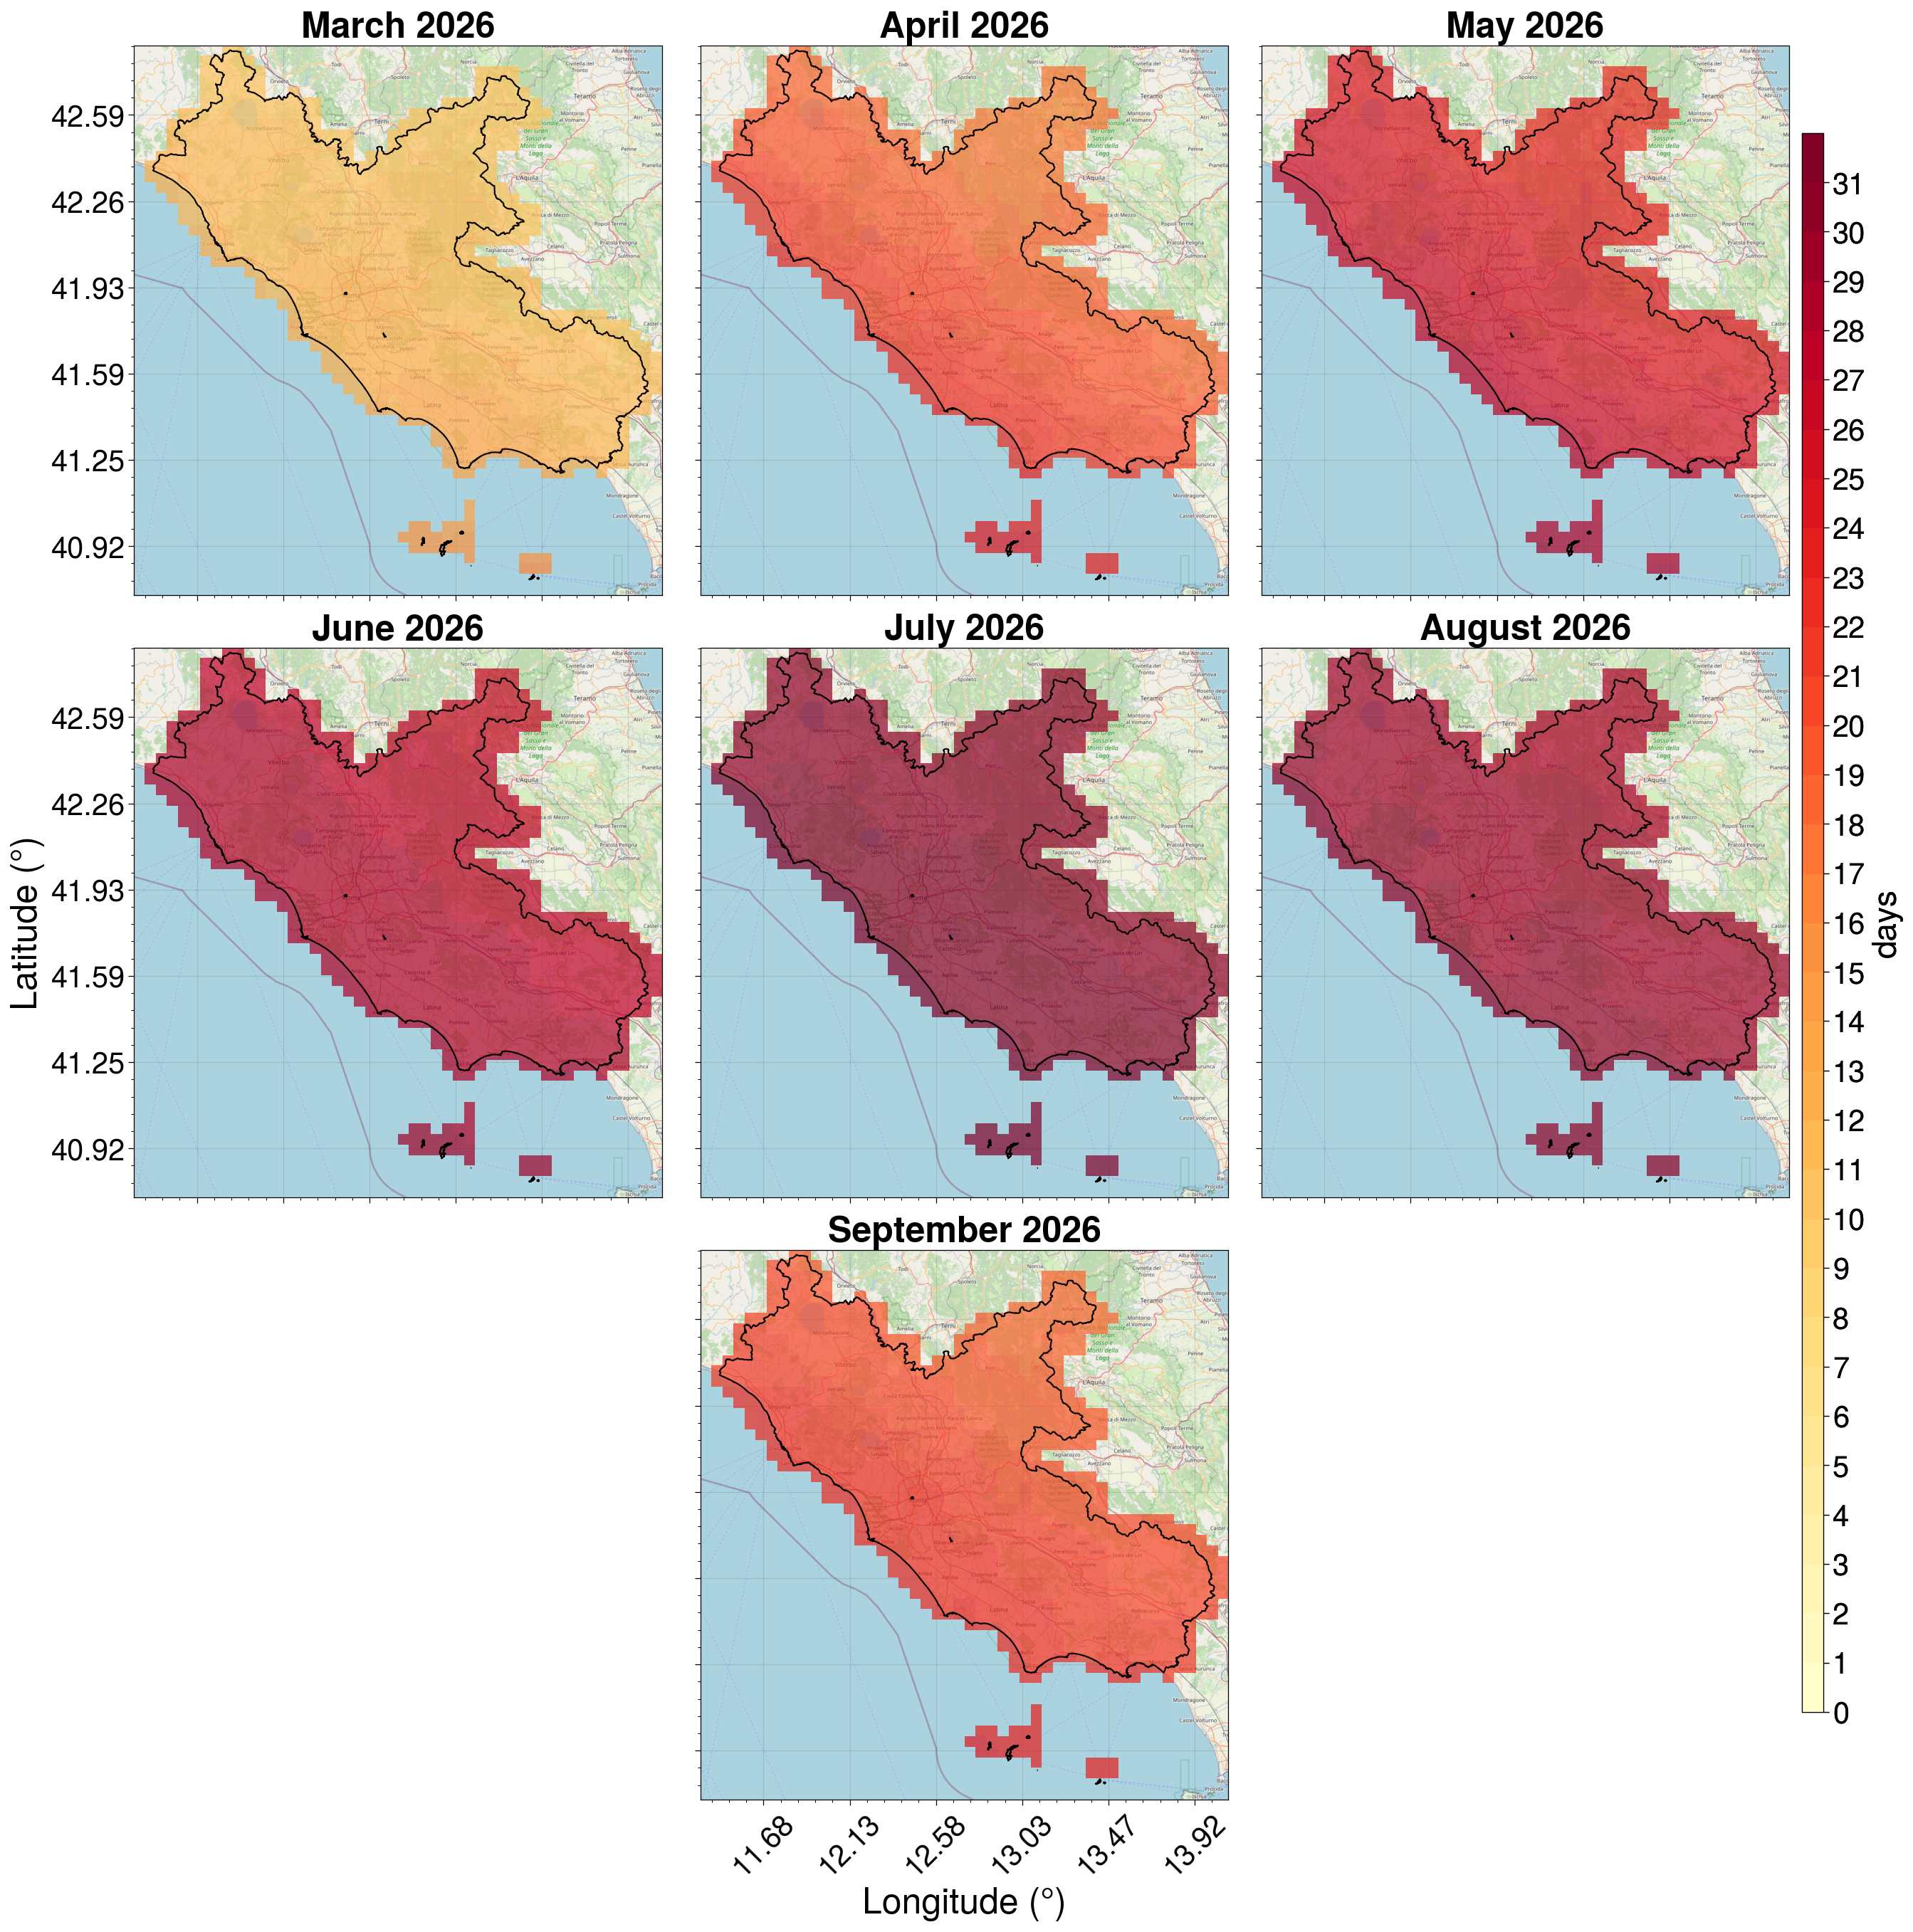
\includegraphics[width=0.95\textwidth]{figures/rad/lazio_rad.png}
\caption{Mappa ad alta risoluzione ($5.5\,\mathrm{km}$) del numero medio di giorni con radiazione solare sufficiente per le operazioni con droni.}
\label{fig: lazio_rad}
\end{figure}
\begin{figure}[H]
\centering
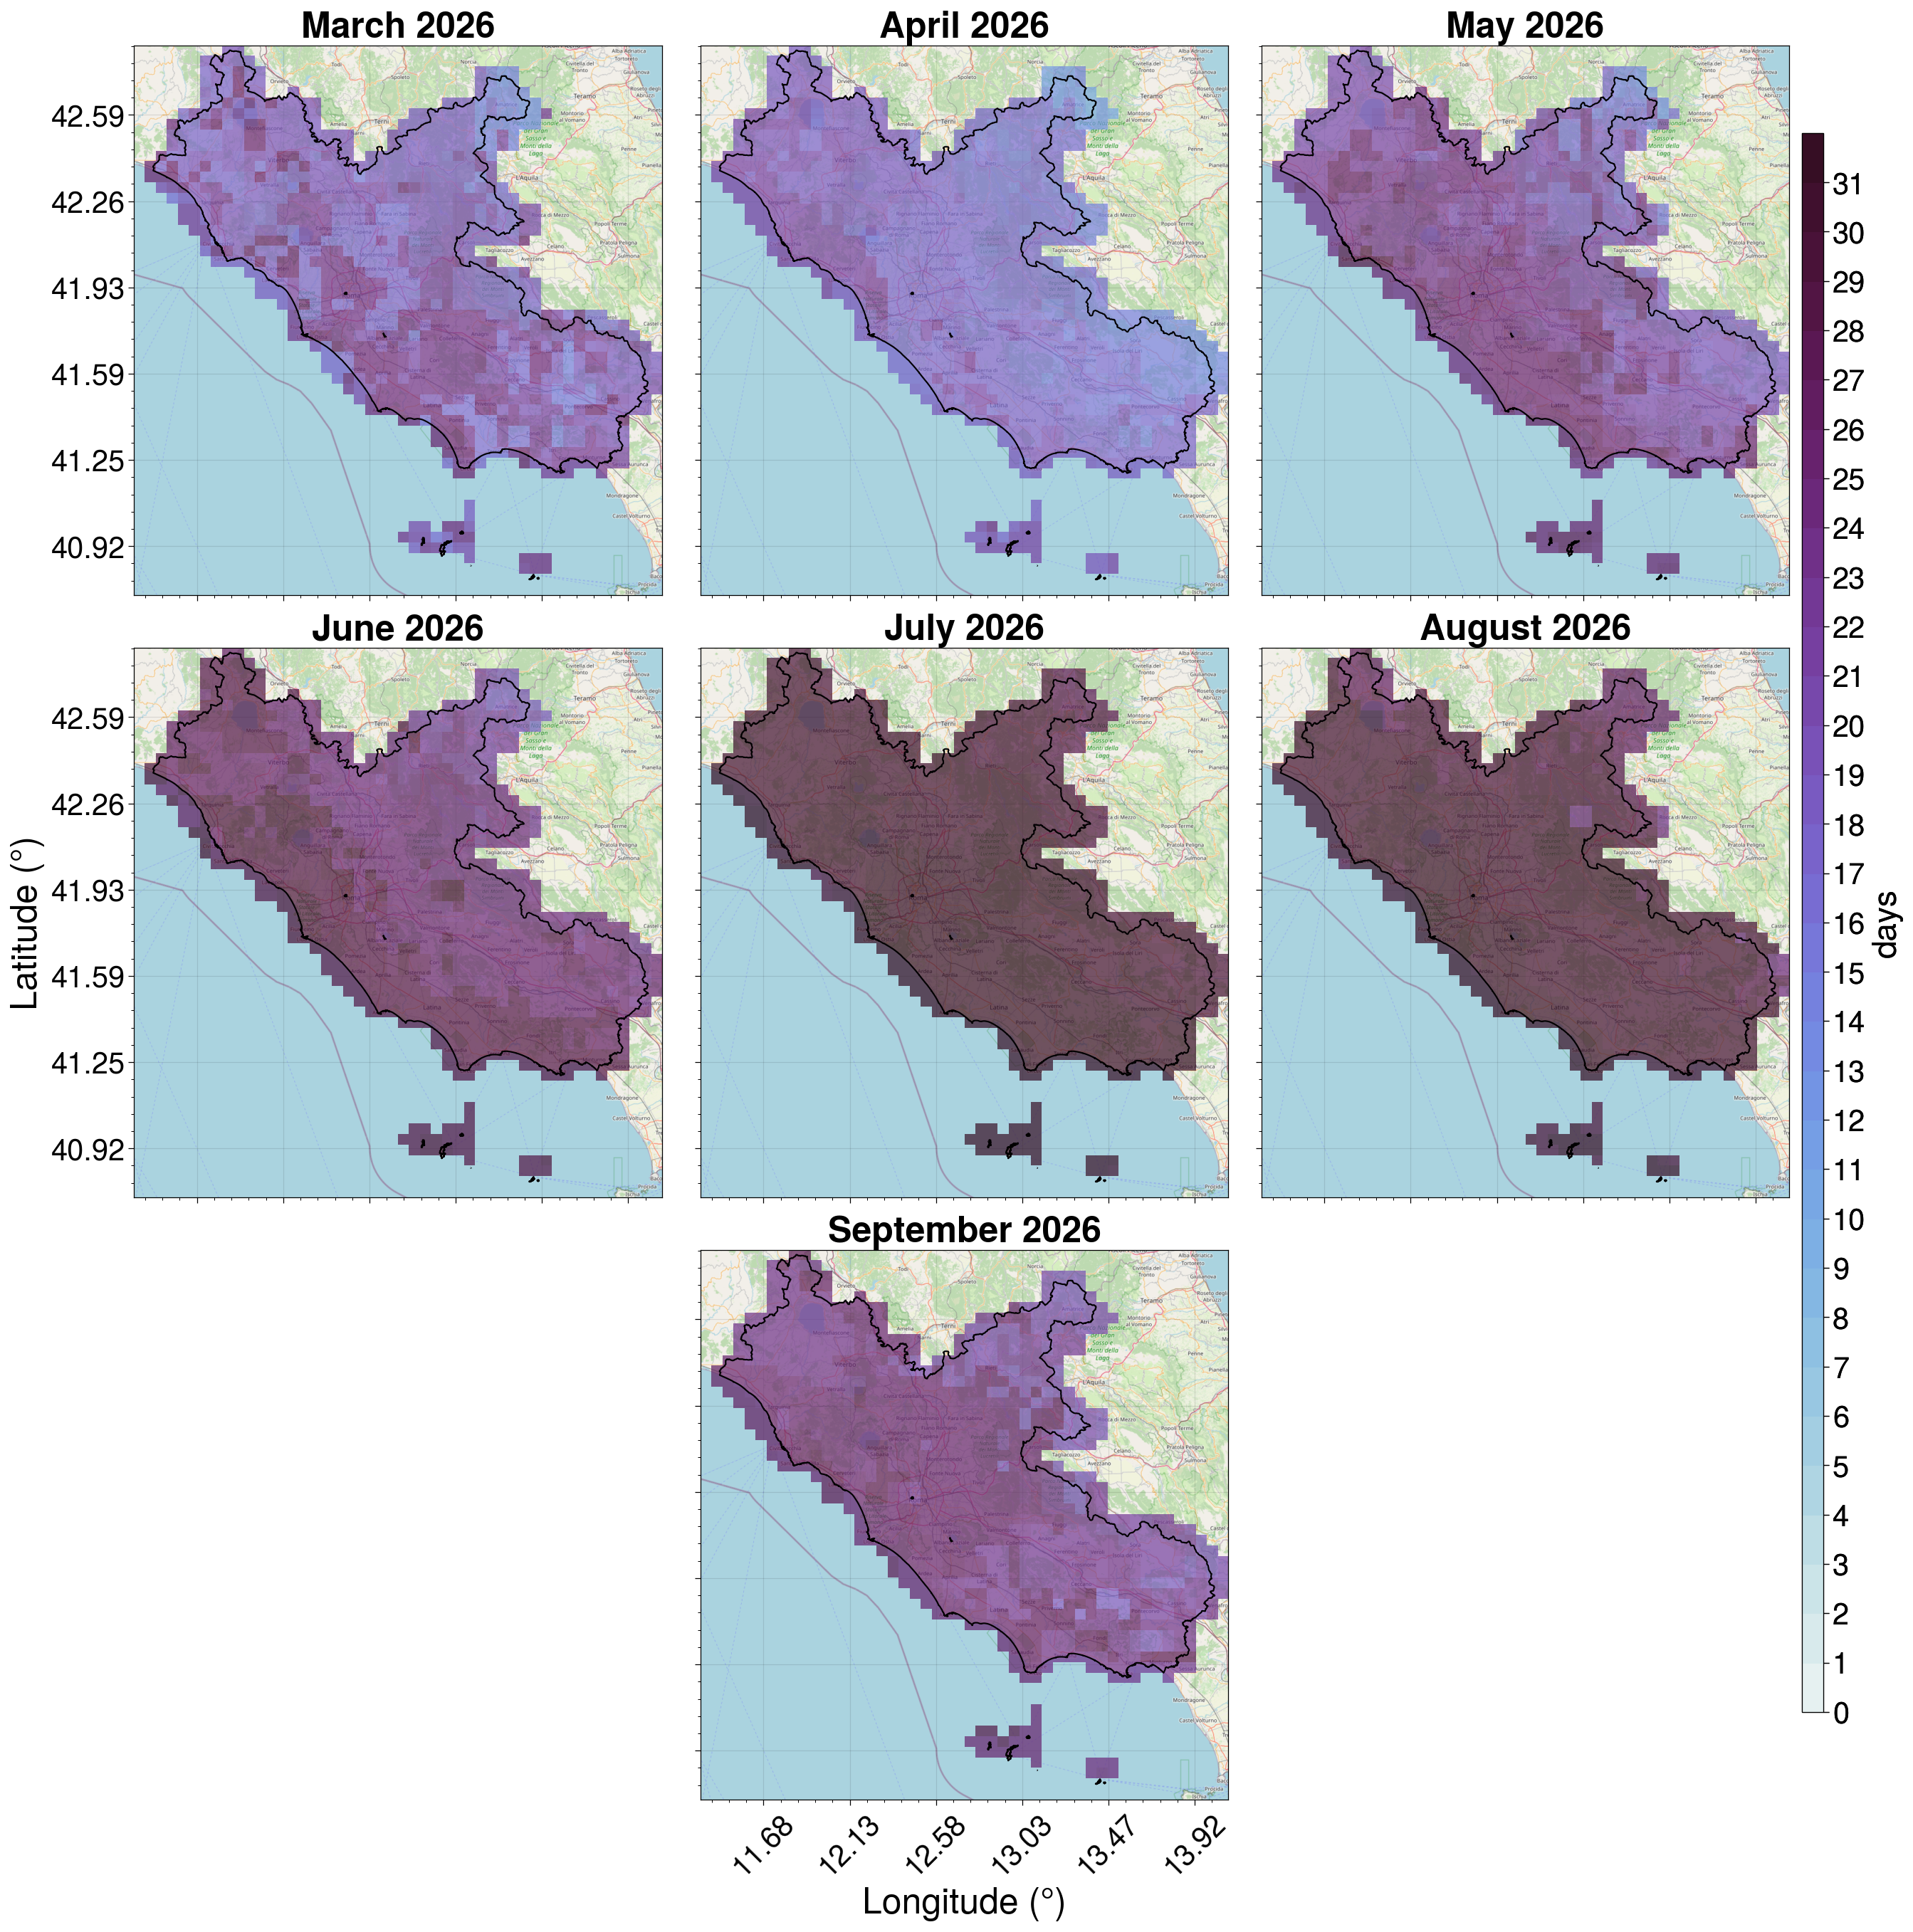
\includegraphics[width=0.95\textwidth]{figures/tp/lazio_tp.png}
\caption{Mappa ad alta risoluzione ($5.5\,\mathrm{km}$) del numero medio di giorni con precipitazione compatibile con le operazioni con droni.}
\label{fig: lazio_tp}
\end{figure}

\subsection{Marche}
\begin{figure}[H]
\centering
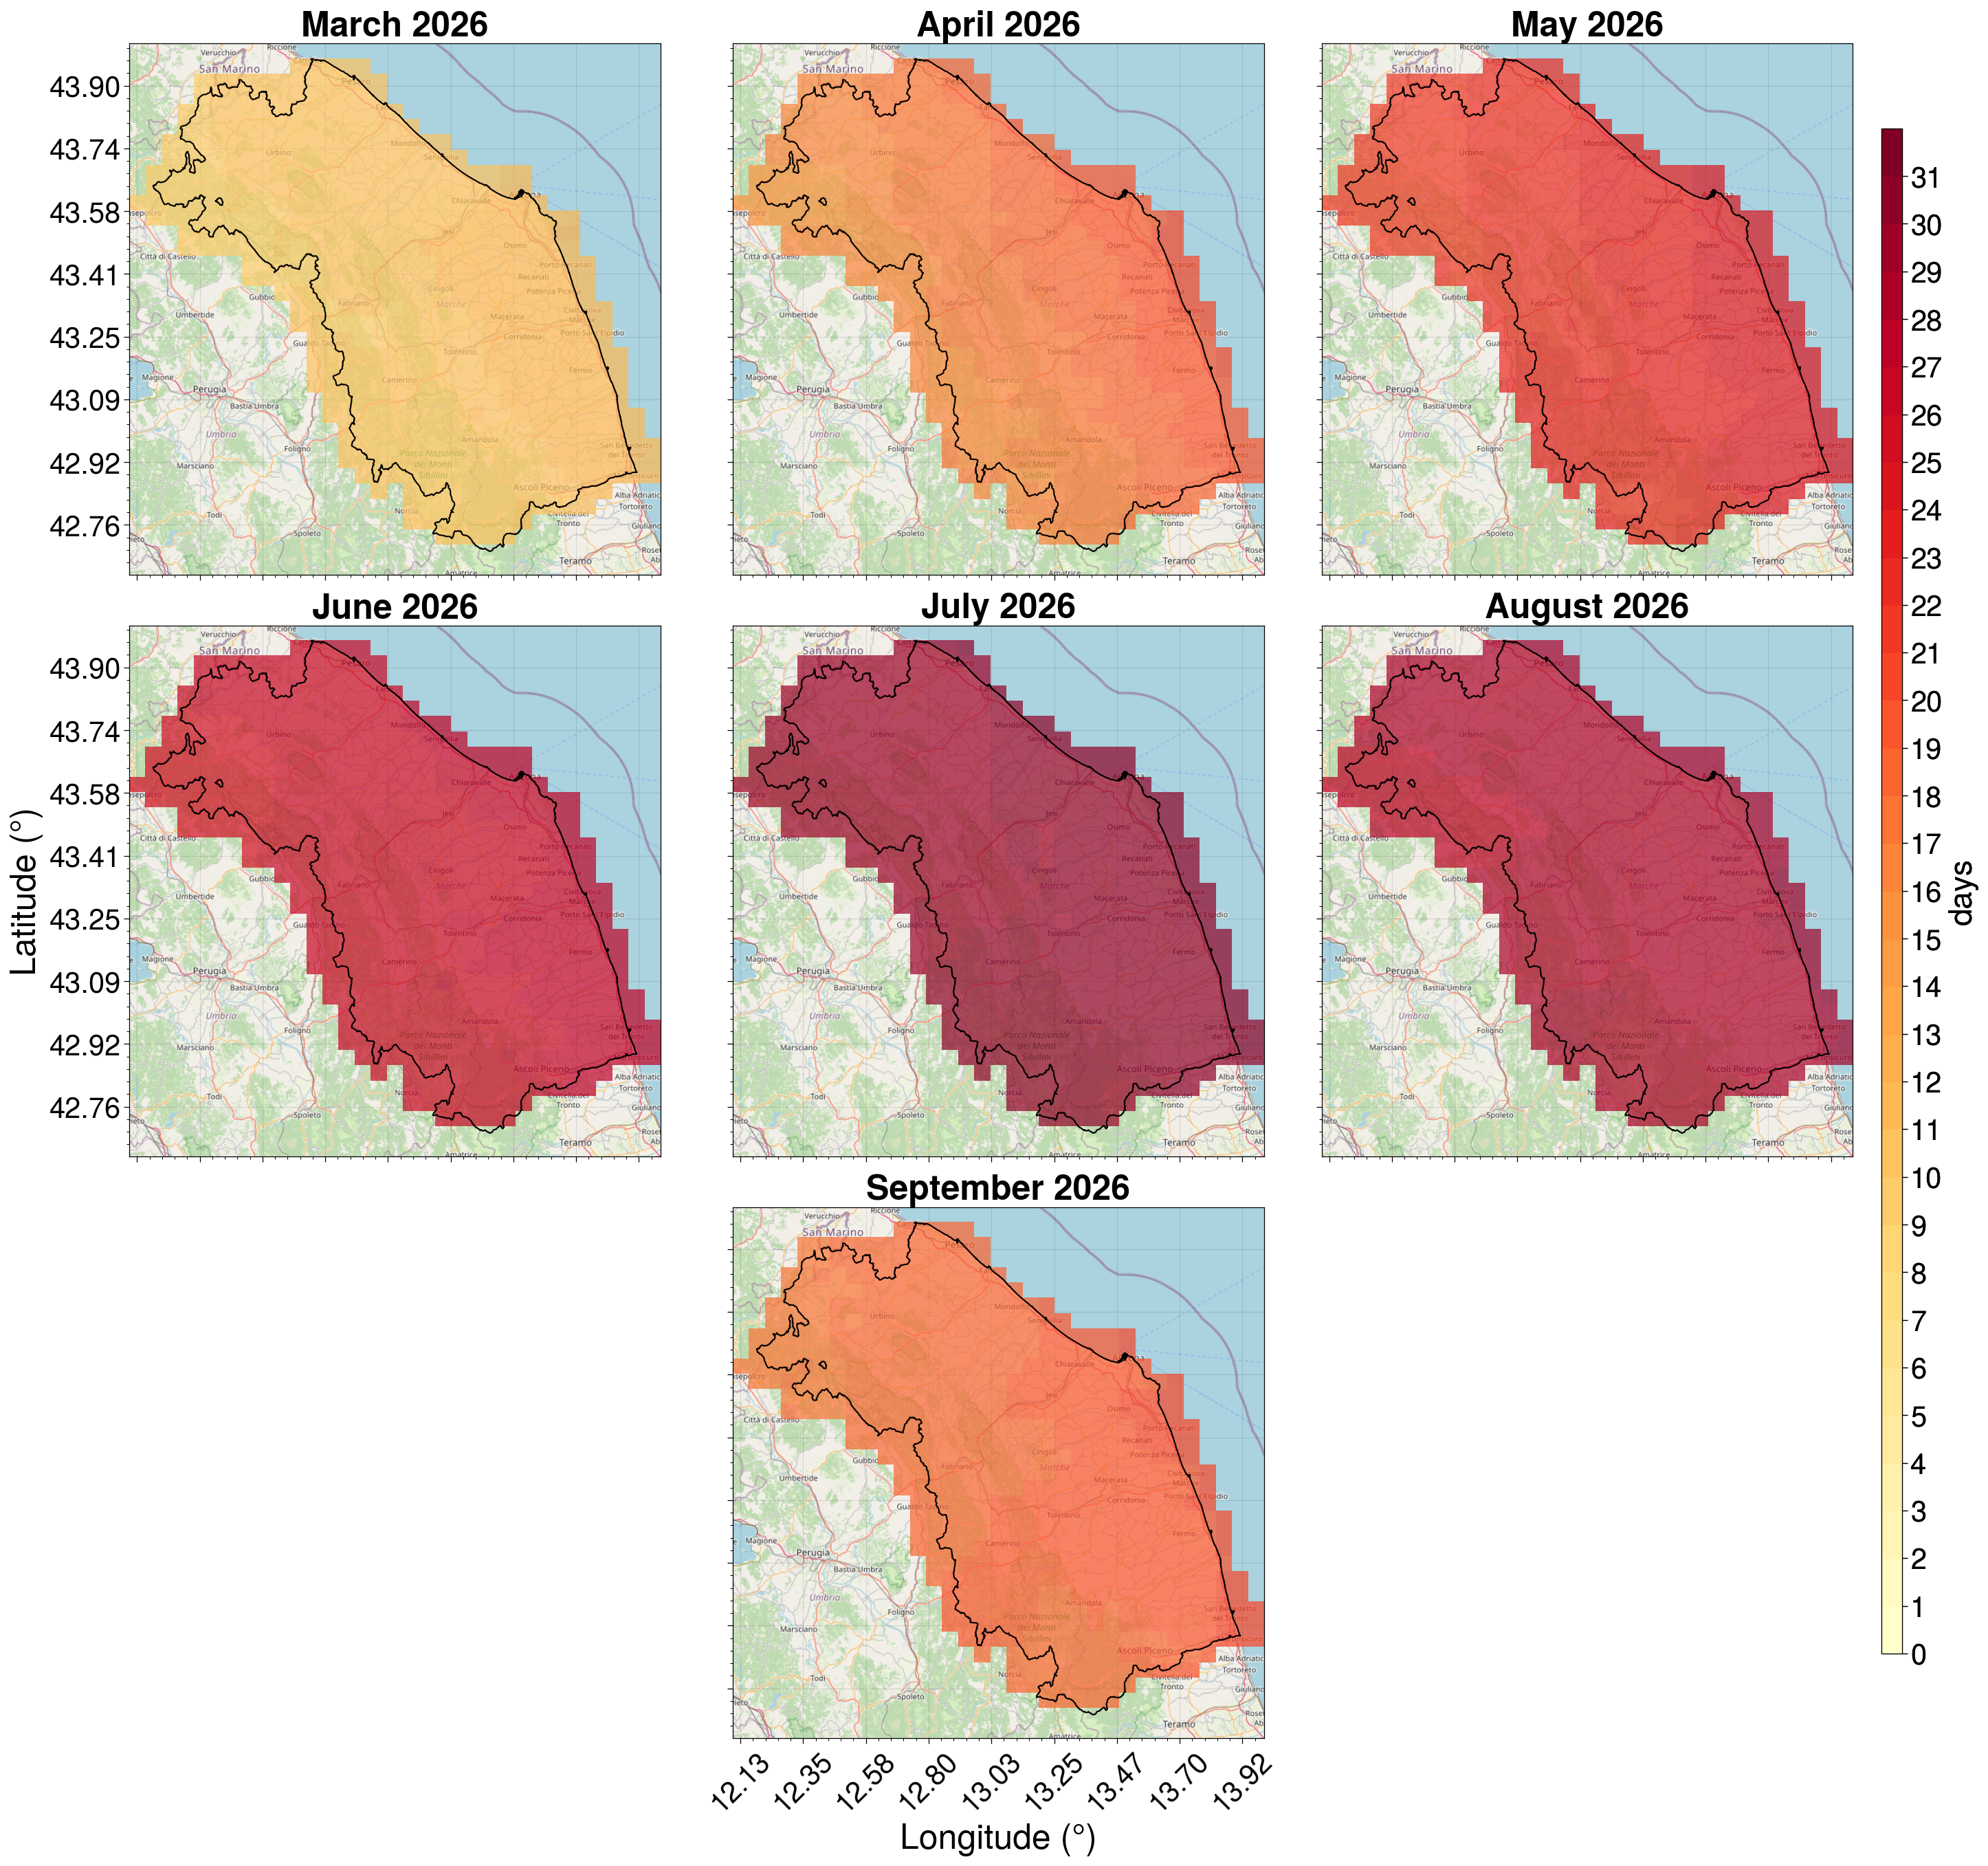
\includegraphics[width=0.95\textwidth]{figures/rad/marche_rad.png}
\caption{Mappa ad alta risoluzione ($5.5\,\mathrm{km}$) del numero medio di giorni con radiazione solare sufficiente per le operazioni con droni.}
\label{fig: marche_rad}
\end{figure}
\begin{figure}[H]
\centering
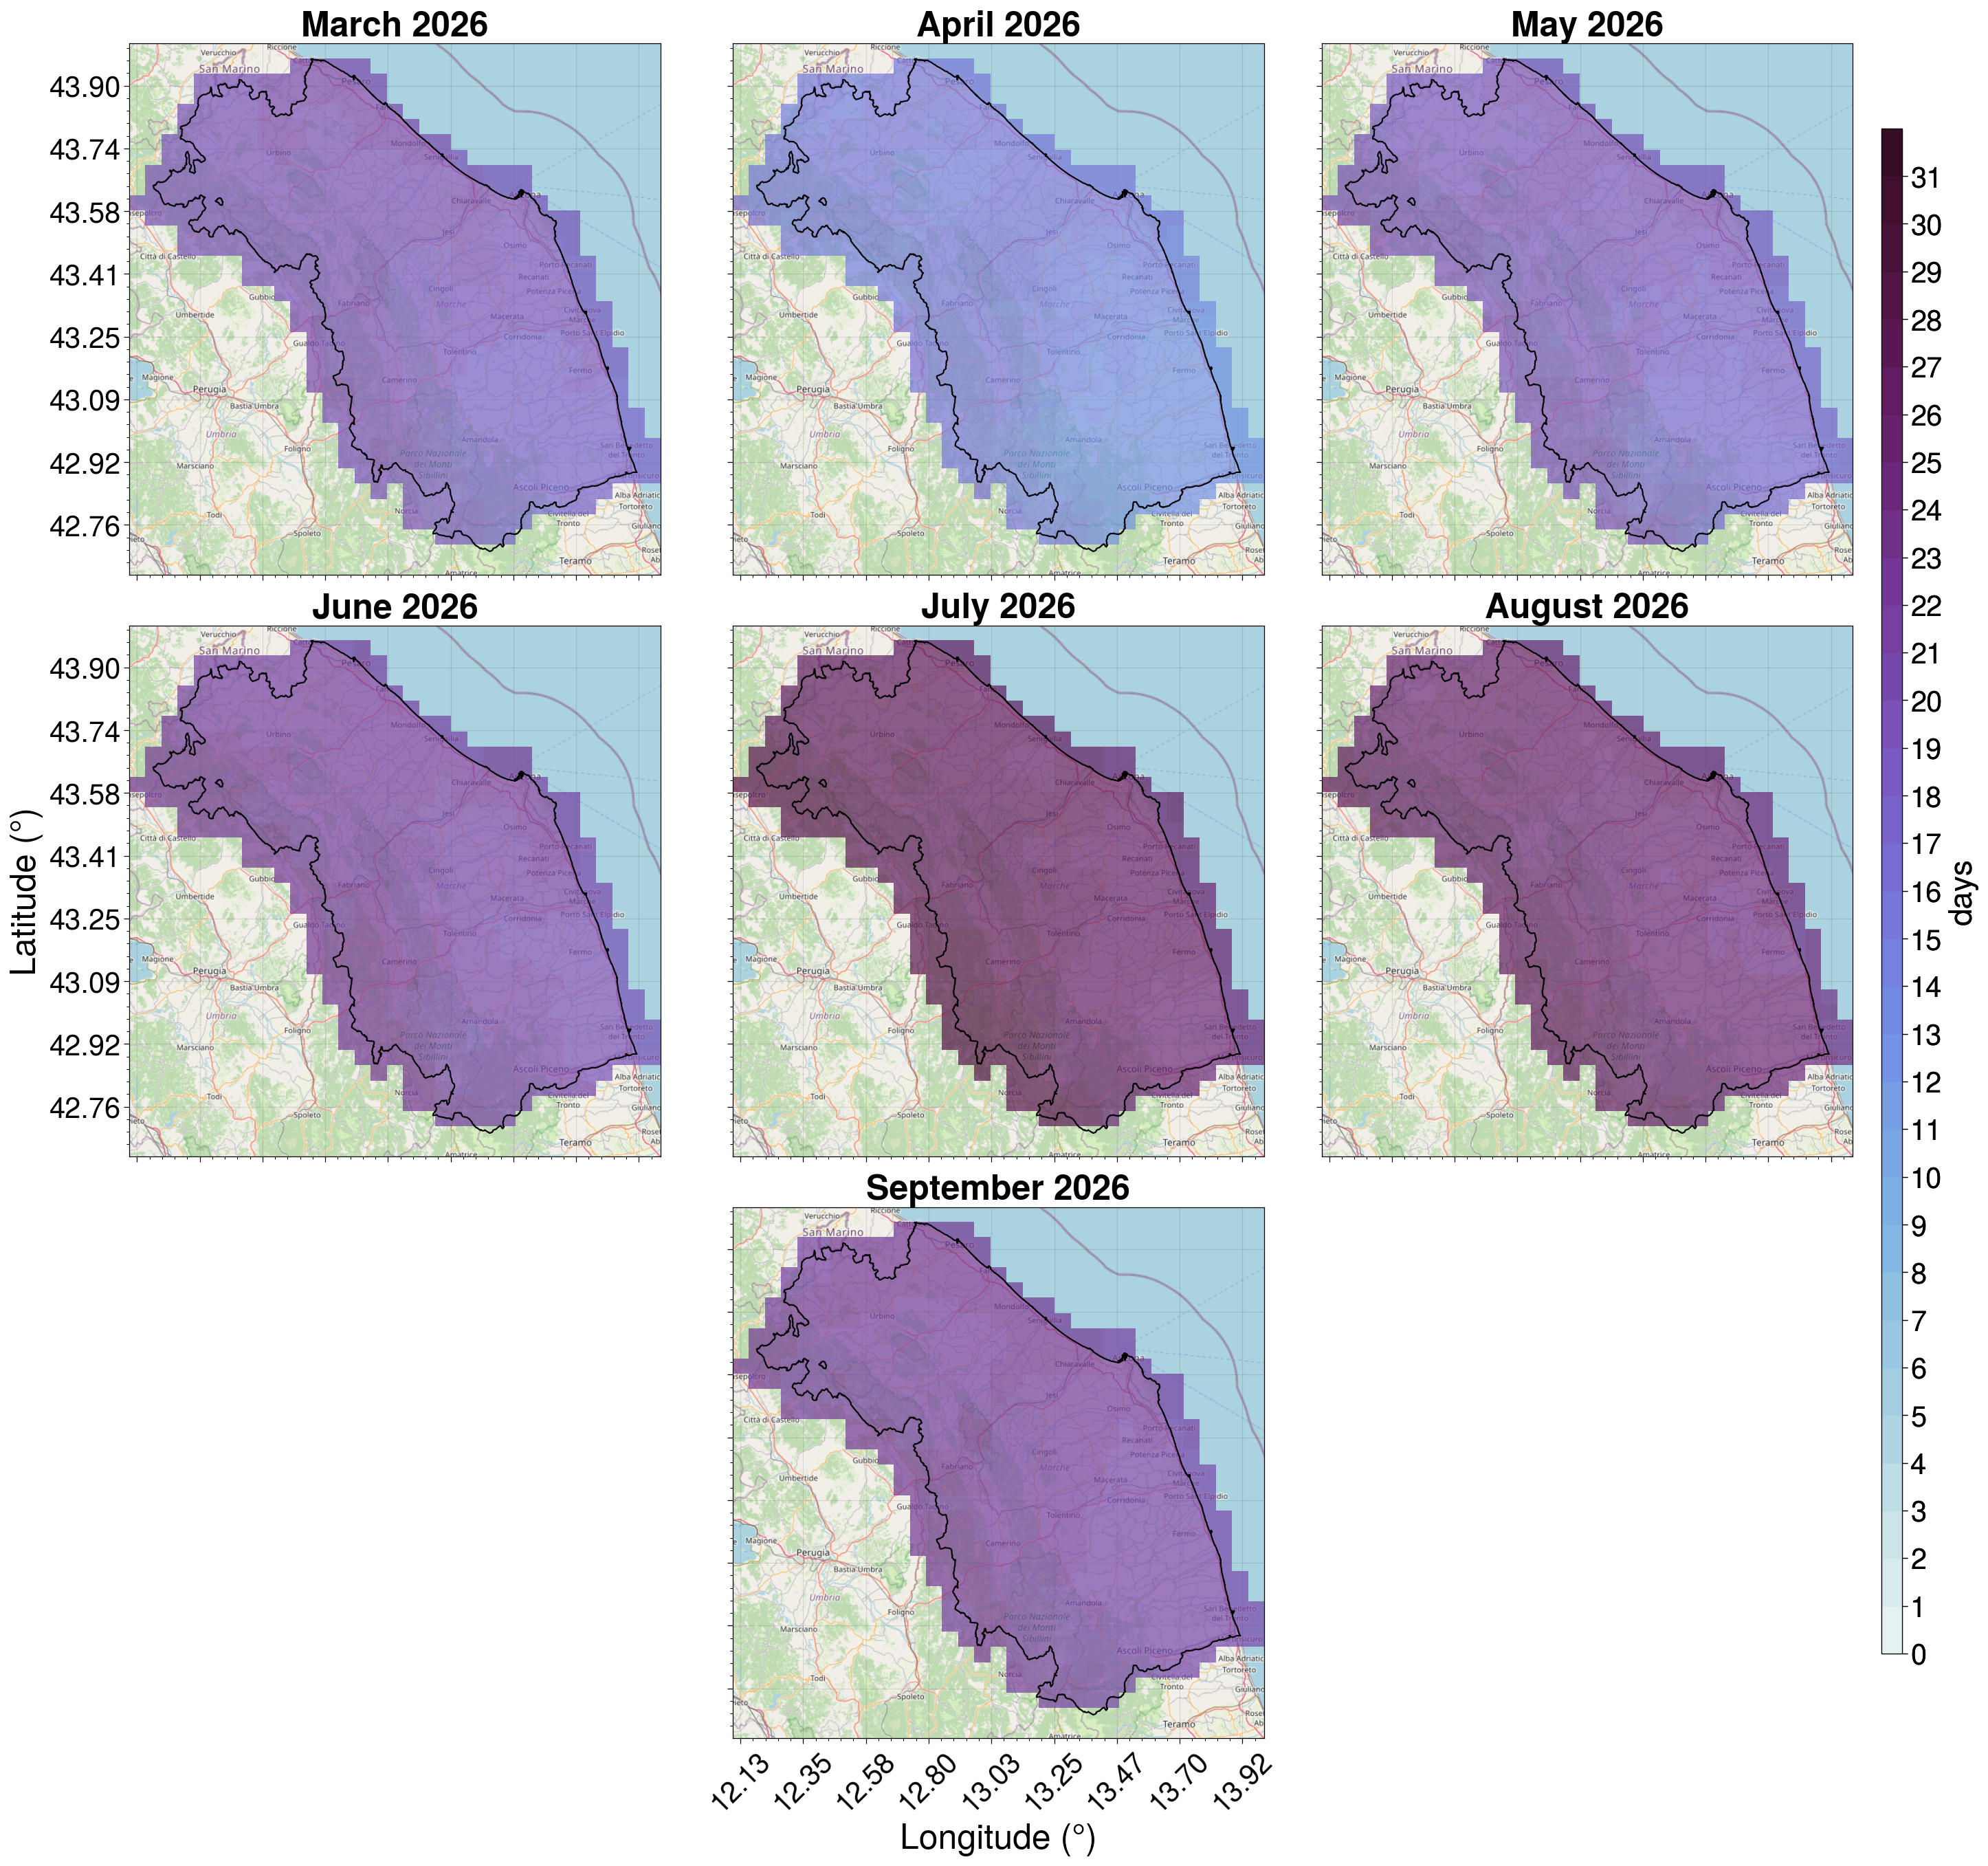
\includegraphics[width=0.95\textwidth]{figures/tp/marche_tp.png}
\caption{Mappa ad alta risoluzione ($5.5\,\mathrm{km}$) del numero medio di giorni con precipitazione compatibile con le operazioni con droni.}
\label{fig: marche_tp}
\end{figure}

\subsection{Piemonte}
\begin{figure}[H]
\centering
\includegraphics[width=0.95\textwidth]{figures/rad/piemonte_rad.png}
\caption{Mappa ad alta risoluzione ($5.5\,\mathrm{km}$) del numero medio di giorni con radiazione solare sufficiente per le operazioni con droni.}
\label{fig: piemonte_rad}
\end{figure}
\begin{figure}[H]
\centering
\includegraphics[width=0.95\textwidth]{figures/tp/piemonte_tp.png}
\caption{Mappa ad alta risoluzione ($5.5\,\mathrm{km}$) del numero medio di giorni con precipitazione compatibile con le operazioni con droni.}
\label{fig: piemonte_tp}
\end{figure}

\subsection{Toscana}
\begin{figure}[H]
\centering
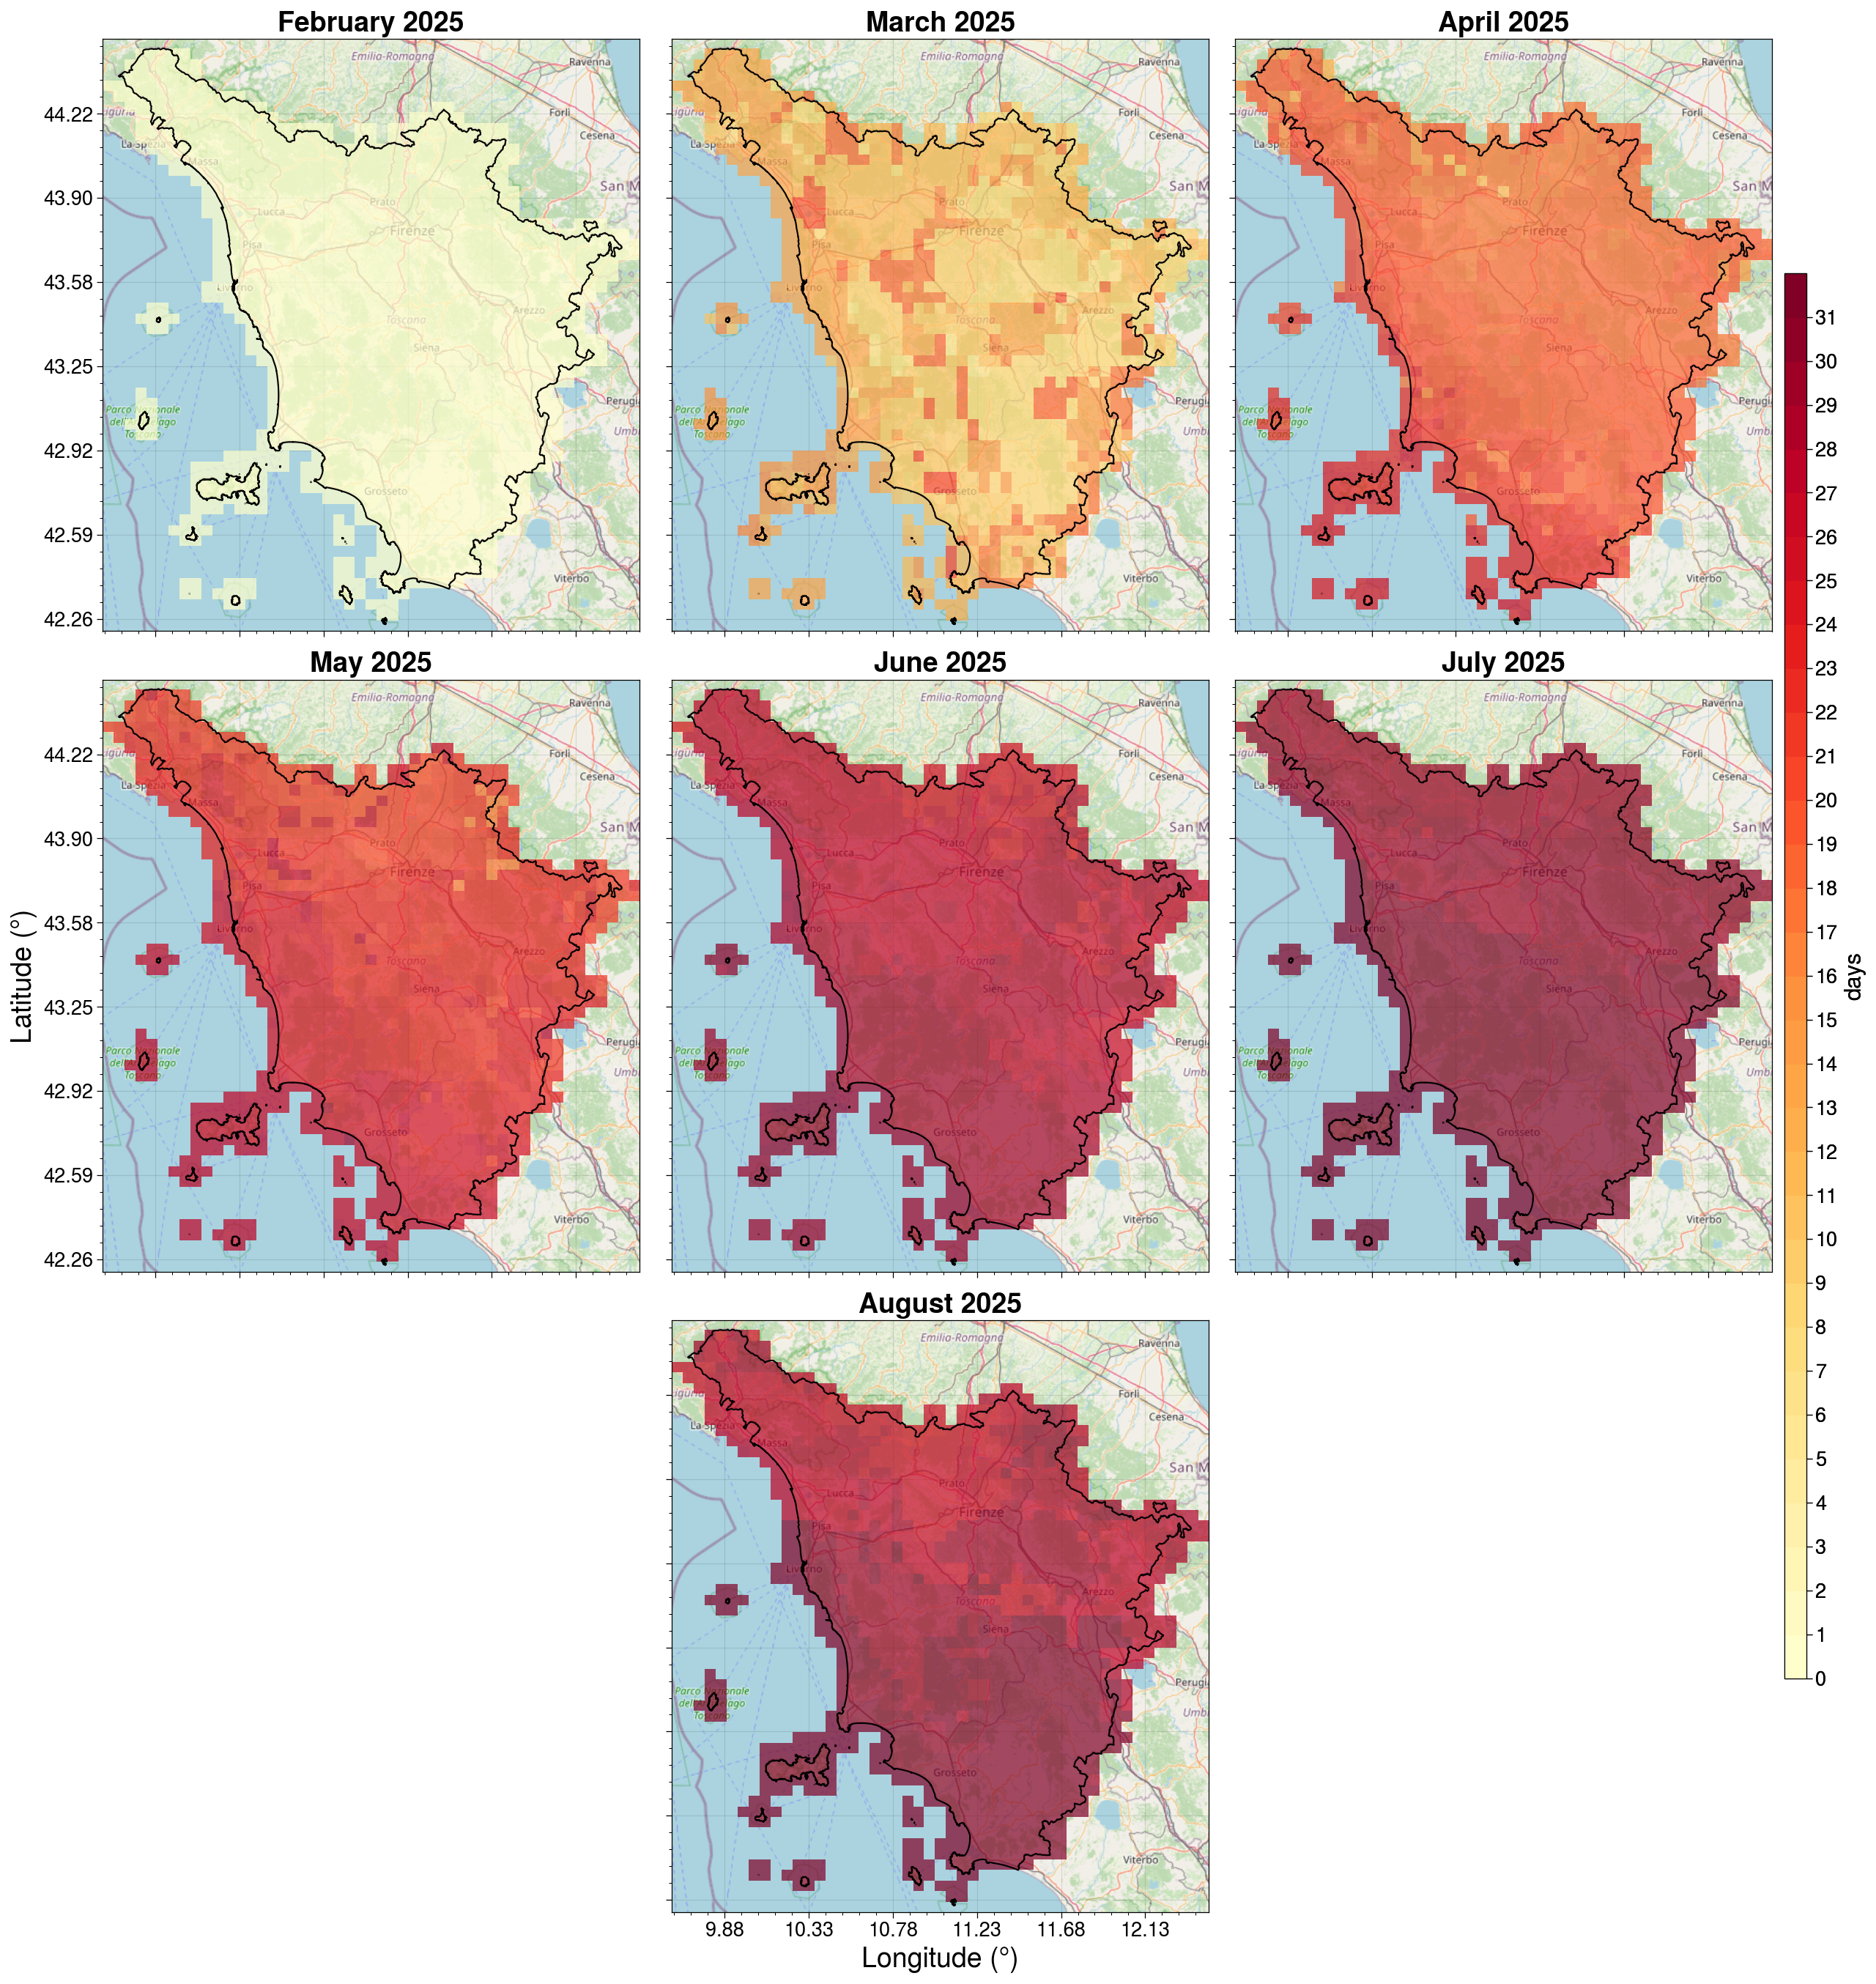
\includegraphics[width=0.95\textwidth]{figures/rad/toscana_rad.png}
\caption{Mappa ad alta risoluzione ($5.5\,\mathrm{km}$) del numero medio di giorni con radiazione solare sufficiente per le operazioni con droni.}
\label{fig: toscana_rad}
\end{figure}
\begin{figure}[H]
\centering
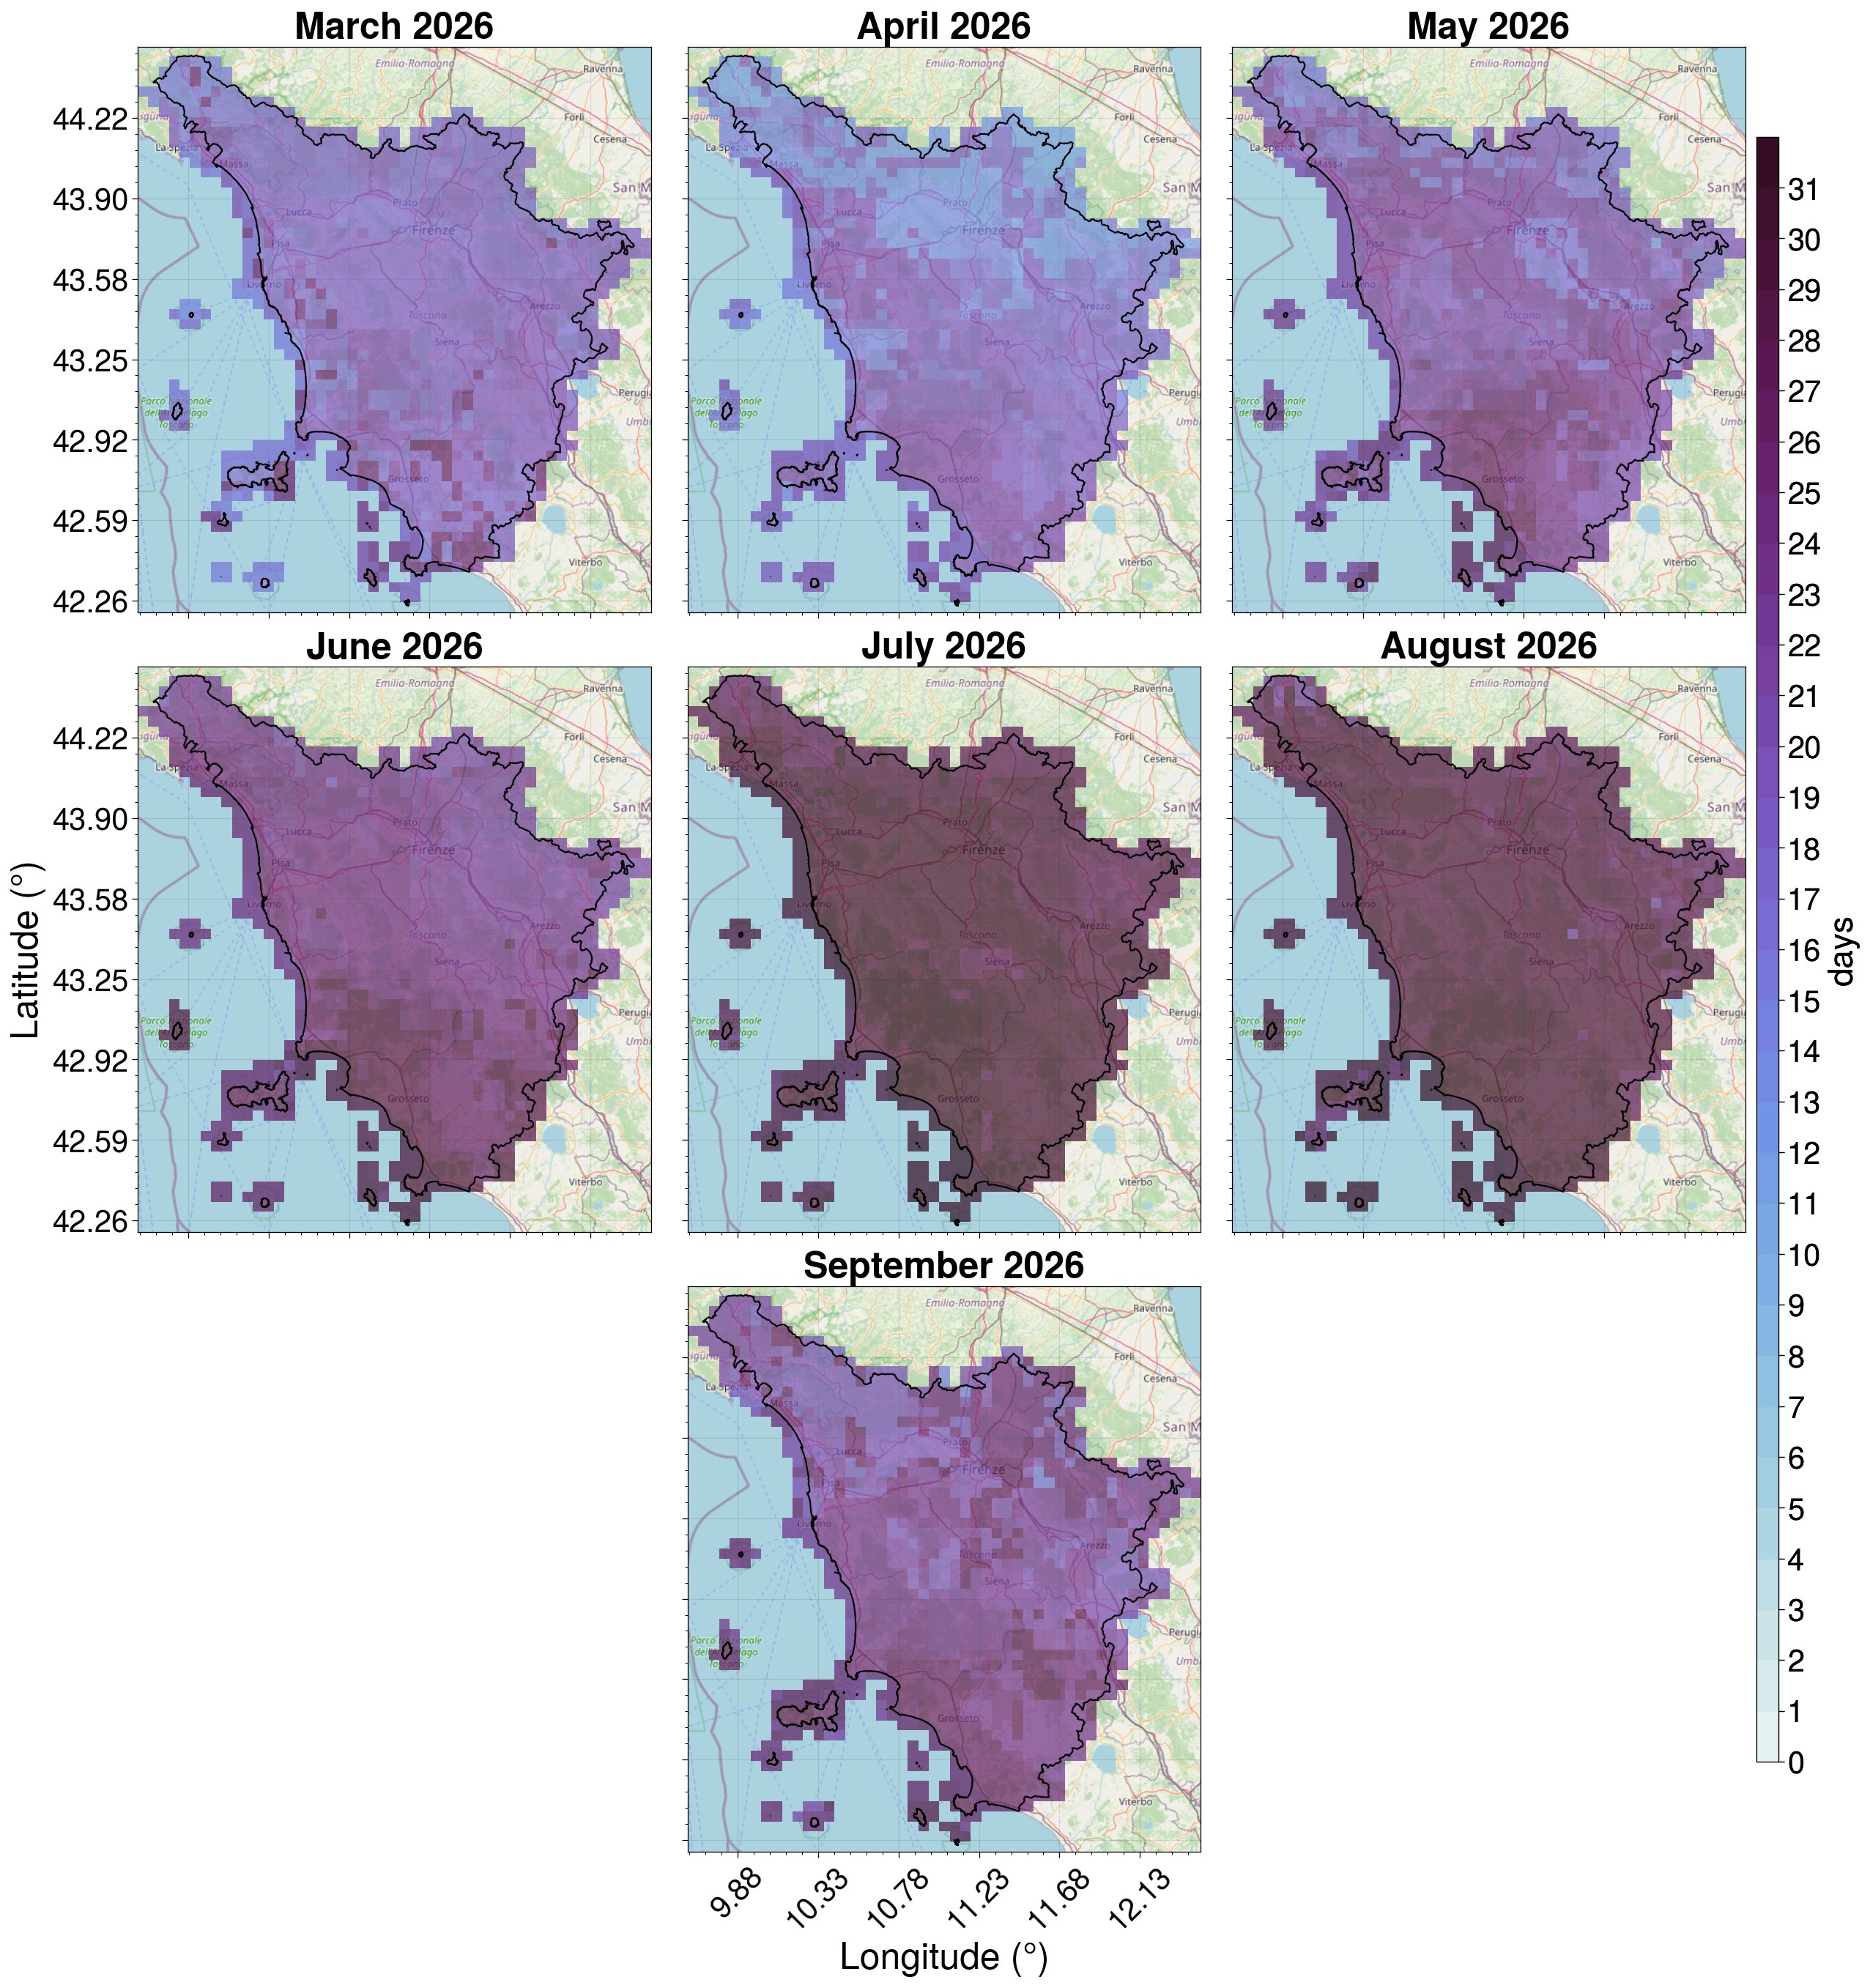
\includegraphics[width=0.95\textwidth]{figures/tp/toscana_tp.png}
\caption{Mappa ad alta risoluzione ($5.5\,\mathrm{km}$) del numero medio di giorni con precipitazione compatibile con le operazioni con droni.}
\label{fig: toscana_tp}
\end{figure}

\subsection{Umbria}
\begin{figure}[H]
\centering
\includegraphics[width=0.95\textwidth]{figures/rad/umbria_rad.png}
\caption{Mappa ad alta risoluzione ($5.5\,\mathrm{km}$) del numero medio di giorni con radiazione solare sufficiente per le operazioni con droni.}
\label{fig: umbria_rad}
\end{figure}
\begin{figure}[H]
\centering
\includegraphics[width=0.95\textwidth]{figures/tp/umbria_tp.png}
\caption{Mappa ad alta risoluzione ($5.5\,\mathrm{km}$) del numero medio di giorni con precipitazione compatibile con le operazioni con droni.}
\label{fig: umbria_tp}
\end{figure}

\end{document}

